\begin{figure}
\def\vl#1{\draw[color=black,dashed] (#1,0) -- (#1,3);}
\begin{center}
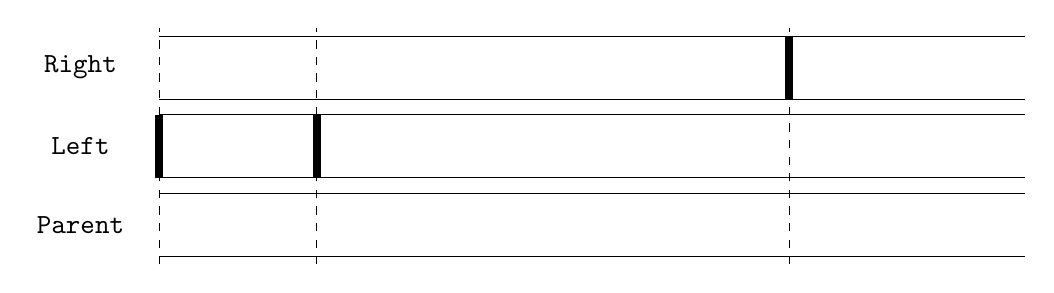
\begin{tikzpicture}
	\draw (0,2.9) -- (11,2.9);
	\draw (0,2.1) -- (11,2.1);
	\draw (0,1.9) -- (11,1.9);	
	\draw (0,1.1) -- (11,1.1);
	\draw (0,0.9) -- (11,0.9);
	\draw (0,0.1) -- (11,0.1);
	
	\vl{0}
	\vl{2}
	\vl{8}
	
	\draw[line width = 1mm] (0,1.1) -- (0,1.9);
	\draw[line width = 1mm] (2,1.1) -- (2,1.9);
	\draw[line width = 1mm] (8,2.1) -- (8,2.9);
	
	\node at (-1,0.5) {\tt Parent};
	\node at (-1,1.5) {\tt Left};
	\node at (-1,2.5) {\tt Right};
\end{tikzpicture}
\vspace{10mm}

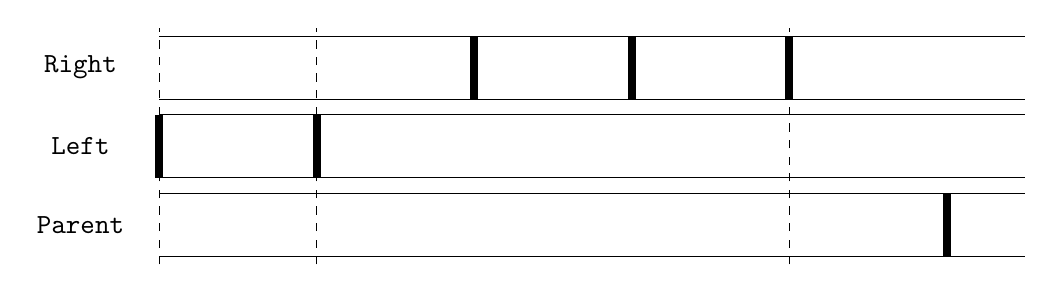
\begin{tikzpicture}
	\draw (0,2.9) -- (11,2.9);
	\draw (0,2.1) -- (11,2.1);
	\draw (0,1.9) -- (11,1.9);	
	\draw (0,1.1) -- (11,1.1);
	\draw (0,0.9) -- (11,0.9);
	\draw (0,0.1) -- (11,0.1);
	
	\vl{0}
	\vl{2}
	\vl{8}
	
	\draw[line width = 1mm] (0,1.1) -- (0,1.9);
	\draw[line width = 1mm] (2,1.1) -- (2,1.9);
	\draw[line width = 1mm] (8,2.1) -- (8,2.9);
	\draw[line width = 1mm] (4,2.1) -- (4,2.9);
	\draw[line width = 1mm] (6,2.1) -- (6,2.9);
	\draw[line width = 1mm] (10,0.1) -- (10,0.9);
	
	\node at (-1,0.5) {\tt Parent};
	\node at (-1,1.5) {\tt Left};
	\node at (-1,2.5) {\tt Right};
\end{tikzpicture}
\vspace{10mm}

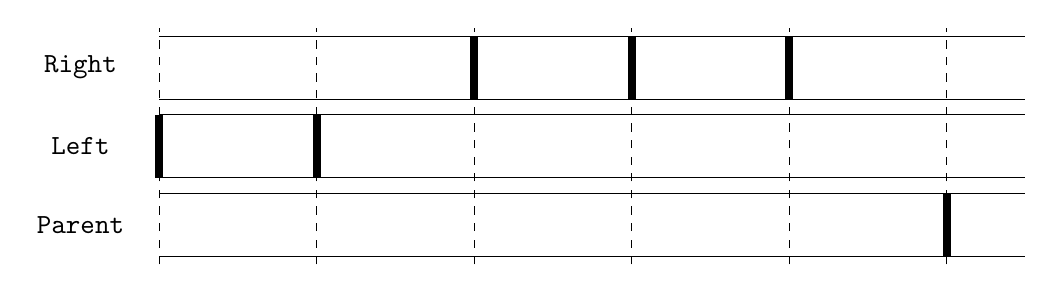
\begin{tikzpicture}
	\draw (0,2.9) -- (11,2.9);
	\draw (0,2.1) -- (11,2.1);
	\draw (0,1.9) -- (11,1.9);	
	\draw (0,1.1) -- (11,1.1);
	\draw (0,0.9) -- (11,0.9);
	\draw (0,0.1) -- (11,0.1);
	
	\vl{0}
	\vl{2}
	\vl{4}
	\vl{6}
	\vl{8}
	\vl{10}
	
	\draw[line width = 1mm] (0,1.1) -- (0,1.9);
	\draw[line width = 1mm] (2,1.1) -- (2,1.9);
	\draw[line width = 1mm] (8,2.1) -- (8,2.9);
	\draw[line width = 1mm] (4,2.1) -- (4,2.9);
	\draw[line width = 1mm] (6,2.1) -- (6,2.9);
	\draw[line width = 1mm] (10,0.1) -- (10,0.9);
	
	\node at (-1,0.5) {\tt Parent};
	\node at (-1,1.5) {\tt Left};
	\node at (-1,2.5) {\tt Right};
\end{tikzpicture}
\vspace{10mm}

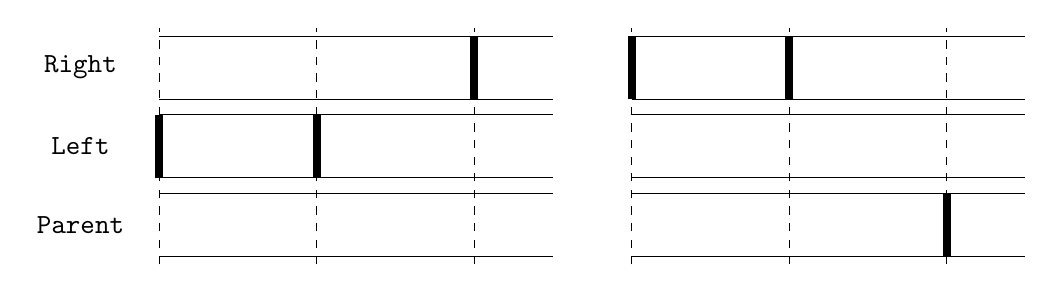
\begin{tikzpicture}
	\draw (0,2.9) -- (5,2.9);
	\draw (0,2.1) -- (5,2.1);
	\draw (0,1.9) -- (5,1.9);	
	\draw (0,1.1) -- (5,1.1);
	\draw (0,0.9) -- (5,0.9);
	\draw (0,0.1) -- (5,0.1);
	
	\draw (6,2.9) -- (11,2.9);
	\draw (6,2.1) -- (11,2.1);
	\draw (6,1.9) -- (11,1.9);	
	\draw (6,1.1) -- (11,1.1);
	\draw (6,0.9) -- (11,0.9);
	\draw (6,0.1) -- (11,0.1);
	
	\vl{0}
	\vl{2}
	\vl{4}
	\vl{6}
	\vl{8}
	\vl{10}
	
	\draw[line width = 1mm] (0,1.1) -- (0,1.9);
	\draw[line width = 1mm] (2,1.1) -- (2,1.9);
	\draw[line width = 1mm] (8,2.1) -- (8,2.9);
	\draw[line width = 1mm] (4,2.1) -- (4,2.9);
	\draw[line width = 1mm] (6,2.1) -- (6,2.9);
	\draw[line width = 1mm] (10,0.1) -- (10,0.9);
	
	\node at (-1,0.5) {\tt Parent};
	\node at (-1,1.5) {\tt Left};
	\node at (-1,2.5) {\tt Right};
\end{tikzpicture}
\vspace{10mm}

\caption{An example of node splitting}
\end{center}
One fat node is depicted in four stages of an update. Intervals of validity of its pointers are indicated by thick vertical lines. Beginning of a slot is illustrated by dashed vertical lines.

In the topmost stage, no changes have been done to the fat node. In the second stage, we see that several fat nodes have been split and there are multiple fat nodes of {\tt Right} and {\tt Parent} corresponding to intervals of one slot. In the third stage we see that additional slots have been created. In the last stage, the fat node has been split in two.
\end{figure}